\documentclass[a4paper,12pt,twoside]{article}
\usepackage[polish]{babel}
\usepackage[utf8]{inputenc}
\usepackage[T1]{fontenc}
\usepackage{graphicx}
\usepackage{anysize}
\usepackage{enumerate}
\usepackage{fancyhdr}
\usepackage{float}
\usepackage{tikz}

\begin{document}

\begin{figure}[!htb]
\centering
\begin{tikzpicture}
\node at (0,0) {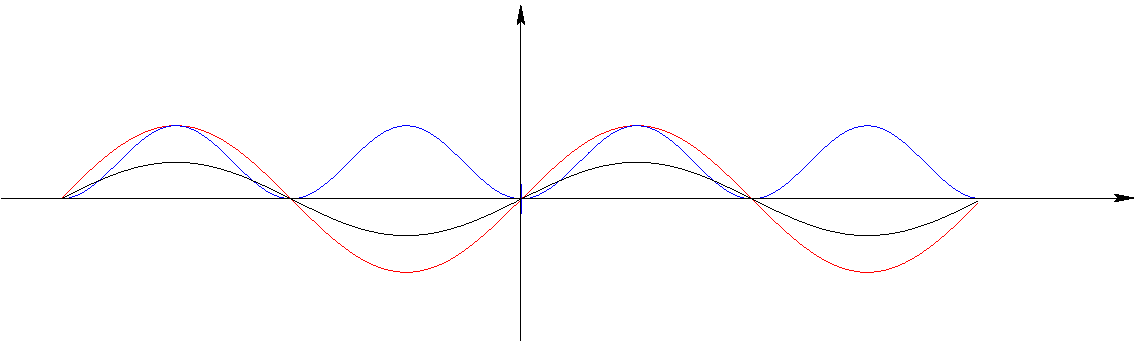
\includegraphics[scale=0.8]{Diagram5}};
\node at (4.1,-1.6) {$f(x) = \sin(x)$};
\node at (4.1, 0.9) {$g(x) = \sin^{2}(x)$};
\node at (1.0, -0.7) {$h(x) = \frac{\sin(x)}{2}}$};
\end{tikzpicture}
\caption{Wykresy funkcji}
\label{fig:funkcje}
\end{figure}

\end{document}